%\documentclass[a4paper,12pt,footexclude,headerexclude]{scrartcl}
%\documentclass{rspublic}  
%\documentclass[conference,abstract,a4paper]{IEEEtran}
\documentclass[a4paper,10pt]{article} 
\usepackage[utf8]{inputenc}
\usepackage{graphicx}
\usepackage{url}
\usepackage{float}
\usepackage{times}    
\usepackage{multirow}    
\usepackage{listings}   
\usepackage{times}     
\usepackage{paralist}
      
\usepackage{typearea}
\areaset[0mm]{6.0in}{8.5in}

% \textwidth = 6.0in
% \textheight = 9.0in
% \oddsidemargin = 0.0in
% \evensidemargin = 0.0in
% \topmargin = 0.0 in
% \headheight = 0.0 in
% \headsep = 0.0 in    


\title{Reliable Replica Exchange Molecular Dynamics Simulation on
  Computational Grids using SAGA-CPR and Migol}

\author{
  Andr\'e Luckow$^{1}$, 
  Shantenu Jha$^{2,3}$, 
  Andre Merzky$^{2}$, \\
  Bettina Schnor$^{1}$ and 
  Joohyun Kim$^{2}$\\
  \small{\emph{$^{1}$Institute of Computer Science, Potsdam University, Germany}}\\
  \small{\emph{$^{2}$Center for Computation \& Technology, Louisiana State University, USA}}\\
  \small{\emph{$^{3}$Department of Computer Science, Louisiana State University, USA}}\\
}

%\date{}

\def\acknowledgementname{Acknowledgements}
\newenvironment{acknowledgement}%
{\section*{\acknowledgementname}%
\parindent=0pt%
}

\bibliographystyle{plain}

 \lstdefinestyle{myC}{
 	language=C,
	basicstyle=\ttfamily \footnotesize,
	breakautoindent=true,
	breaklines=true
  	tabsize=2,
  	captionpos=b
 }

\begin{document} 


\maketitle


% \section*{Introduction}
                           
% Grid computing envisions the sharing of compute, network, data and
% software resources across multiinstitutional virtual organizations
% (VOs). 

Writing applications that are able to orchestrate heterogeneous
resources across virtual organizations (VO) is a complex task.  Several 
classes of applications, which are well suited for loosely
coupled Grids, exist; arguably the best known and most commonly used ones are
task farming applications. Despite the simple nature, many problems
can be solved with such a model, e.\,g.\ parameter studies found in
many sciences or Monte Carlo simulations. More
complicated, but possibly more interesting than {\it pleasingly
  distributed} applications, is the class of applications that are
essentially loosely-coupled, but with a small level of coupling
between the tasks.   A class of algorithms that belongs to this category are
\emph{Replica Exchange Molecular Dynamics (REMD)}~\cite{hansmann,Sugita:1999rm} simulations.
% Replica Exchange~\ref{repex1, repex2} simulations  %reference does not exist in bib
% are a class of algorithms that belong to this category.
% Algorithms that can effectively utilize distributed computing
% infrastructures are often different to those that utilize canonical
% high end computers.  
% Replica exchange (RE) methods~\cite{SPdynamics,
%   pande_bj03} are a class of algorithms that can utilize distributed
% computing infrastructure  
Such simulations are used to understand important physical
phenomena -- ranging from protein folding dynamics to conformational
configuration changes.

The \emph{Simple API for Grid Applications (SAGA)}~\cite{saga_gfd90}
provides a straightforward API for developing loosely coupled data and/or task
parallel applications.
% The framework provides an standardized, easy-to-use 
% API for applications to efficiently utilize Grid infrastructures. 
SAGA offers a standardized, easy to use API for utilizing Grid
infrastructures. The API supports e.\,g.\ the management of Grid jobs,
file transfers and replicas. Thus, SAGA is ideally suited to provide
the orchestration of the of replica exchange simulations across
distributed infrastructure.
                                                         
In replica exchange simulations, there is a need to occasionally attempt an exchange
between pairs of replicas; the pairing of replicas is also not a
constant and is dynamically determined. However, once the pair of
replicas has been established, a delay or loss of one replica will
stall the other replica. In the worst case, a single failing task can
render the entire computation worthless.
\emph{Migol}~\cite{schnorLuckow08} provides a fault tolerant Grid
middleware, which supports the discovery and allocation of resources
as well as the transparent starting, monitoring and recovery of tasks in the Grid.

This paper describes how using the Checkpoint\,\&\,Recovery package
(CPR) of the SAGA API, Migol's fault tolerance can be provided to the
class of Replica Exchange applications.

\section*{Migol \& SAGA CPR: A Fault Tolerant Service Environment for
  Grid Applications}
\label{sec:migol}
\begin{figure}[t]
            \centering
                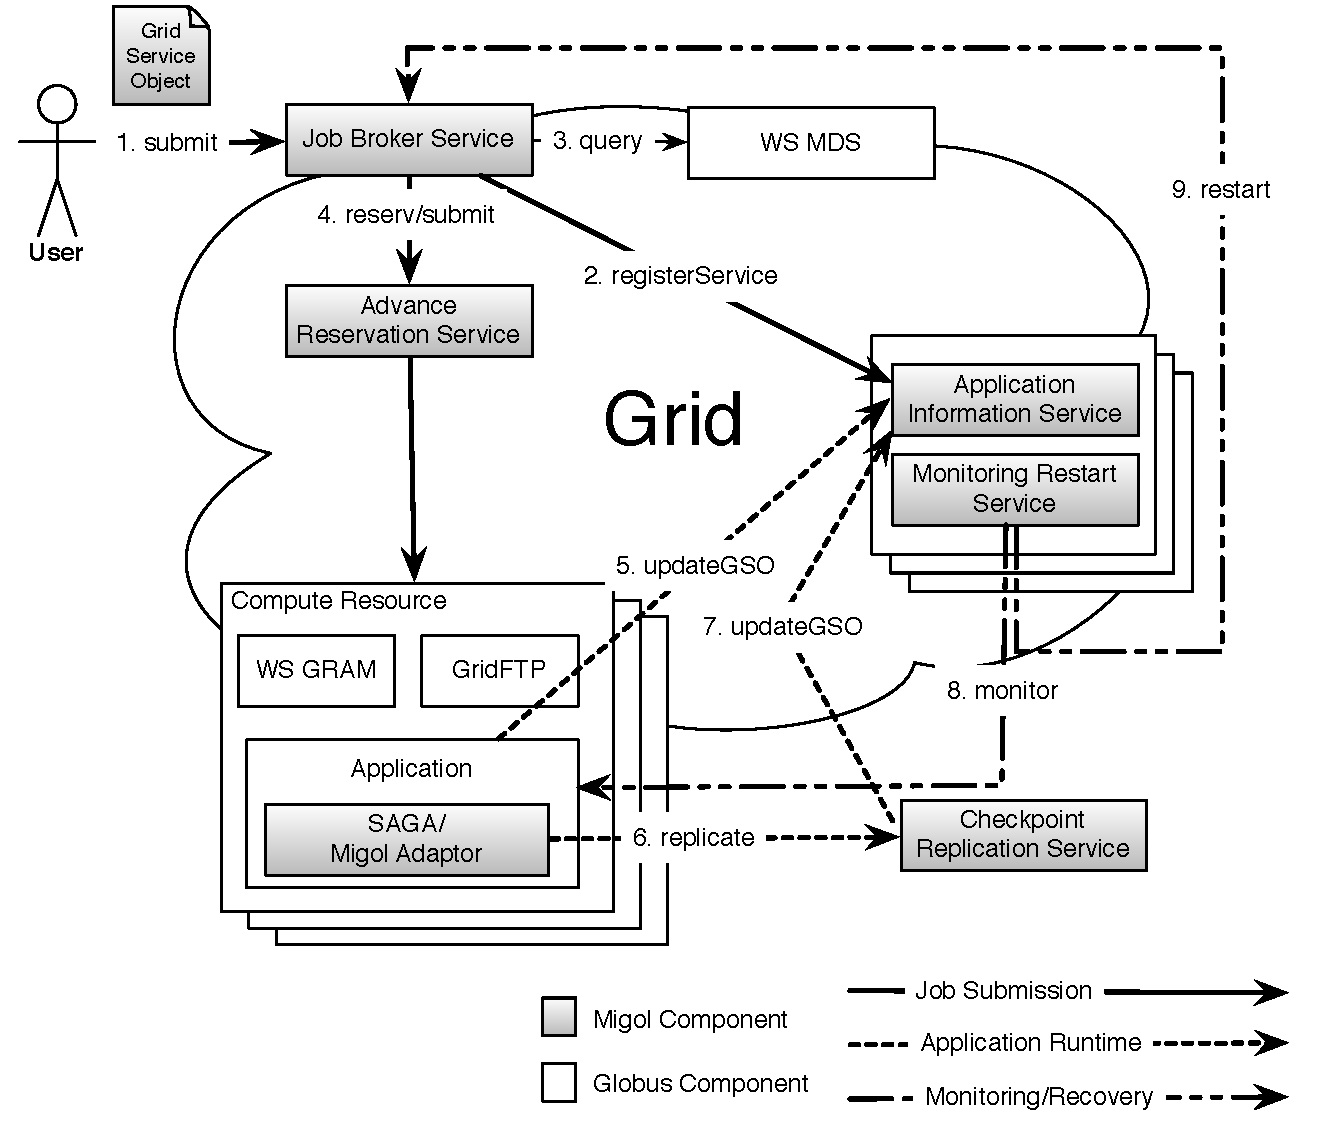
\includegraphics[width=0.7\textwidth]{migol_architecture}
            \caption{Migol Service Architecture and Interactions}
            \label{fig:migol_architecture}
\end{figure}           

Migol guarantees the correct and reliable exe\-cution of applications or tasks even in
the presence of  failures. The framework is based on the Globus Toolkit 4. 
Figure~\ref{fig:migol_architecture} shows the current Migol architecture and 
the interactions between the different services.    
Fault tolerance of applications is achieved by periodically monitoring all applications 
in the Grid using a keep-alive message. Inactive applications are detected via a configurable timeout. In case a failure 
is discovered, a restart respectively a migration is initiated.  For recovery, Migol relies on application-level 
checkpointing, i.\,e.\ applications have to be
written to accommodate checkpointing and restart.    

% The framework has strong self-healing capabilities: critical services, 
% such as the central registry service are replicated and support an automatic reconfiguration.    
                                                                                                          
The new SAGA CPR package provides a clean abstraction for starting,
monitoring and recovering of checkpoint-restartable jobs.
% The package was inspired by the GridCPR~\cite{gridcpr} architecture and Migol.           
Using SAGA CPR, applications can register checkpoint and job metadata with the infrastructure. Further, the API provides support for starting applications, triggering of checkpoints and recoveries.

The aim of this paper is, i) to couple the SAGA and Migol
frameworks, ii) to provide a proof of concept implementation of the
replica exchange method that uses the SAGA/Migol frameworks, iii) to show
the validity, scalability and extensibility of this approach by
attempting the simulation of a large model system.
In the full paper, we will extensively  describe the design of the SAGA CPR API and the implementation 
of the Migol adaptor. Further, we will present our experiences with deploying  
the REMD application in a Grid environment.
                                                                    
%%------------------------------------------------------------------------------
%\section*{Conclusion}         
% Migol addresses the fault tolerance of Grid applications by handling common failures   
% in applications transparently without user interactions.  In case of failures, 
% e.\,g.\ a node-crash, applications are automatically restarted 
% from the last saved checkpoint. The new SAGA Checkpoint Recovery (CPR) API
% provides a clean application-level abstraction to Migol. 


\bibliographystyle{IEEEtran}
\bibliography{saga,literatur}
\end{document}


%TODO Future Work

%Migol provides an integrated solution for the management of data and
%compute resources.

% A main limitation of current Grid infrastructures is the restricted availability of 
% precise resource information. Managing this information uncertainty is difficult and often leads to
% a trial-and-error approach. For example, a transfer service cannot 
% differentiate between a harddisk failure and a transient network failure. While a retry 
% will resolve a transient failure, in case of a harddisk failure this approach will very likely not be successful.
% An adaptive strategy for tuning fault detection timeouts is therefore essential to achieve a 
% sufficient reliable fault detection while maintaining an acceptable performance.        

% Granularity of SAGA API not always well suited for Grid service interactions.
%%------------------------------------------------------------------------------     




% \begin{abstract}   {Grid Computing, Task Farming, SAGA, Migol}
% A major challenge in a dynamic Grid with thousands of machines connected to
% each other is fault tolerance. The more resources and components involved, the
% more complicated and error-prone becomes the system. 
% Migol~\cite{schnorLuckow08} is an adaptive Grid middleware,
% which addresses the fault tolerance of Grid applications and services 
% by providing the capability to recover applications from checkpoint files 
% transparently. 
% 
% SAGA~\cite{SAGA_Goodale06a} provides a standardized, application-level API for 
% common Grid scenarios, e.\,g.\
% the management of files and jobs. The new SAGA Checkpoint Recovery (CPR) package addresses checkpointing 
% and the automatic recovery of Grid applications. In this paper, we describe the design of 
% the SAGA CPR package, the integration of the CPR adaptor with the Migol infrastructure, 
% and our experiences with running a large scale SAGA CPR based task farming application 
% in a real Grid environment. 
% \end{abstract}   

%%------------------------------------------------------------------------------
% Open Topics:
% How long running are Map-Reduce sorting problems?
% Sorting with MapReduce: 1TB data => runtime 891 s (Dean, Google)
% SAGA provides a more low level primitives than Hadoop or Google MapReduce.
% What failure detection timeouts per task should be used?
% Performance measurement: without versus with failures    
% Comparison w/ Google MapReduce infrastructure:
%         - Master responsible for allocating mapper tasks (close to data)   
% Limitations of SAGA map-reduce
%       - low-level handling of file transfers and jobs required (ft aspect can be handled by Migol) 
%       - no sorting of data between map and reduce



% Long-running applications can significantly benefit from Migol:
% Without human interaction, recovery times are minimized, and the
% application and infrastructure utilization is enhanced.  While the
% Google's map-reduce infrastructure is tailored to the special needs
% of Google, SAGA provides an open standard, which allows the
% middleware independent implementation of MapReduce. Migol can
% provide a fault-tolerant run-time for map and reduction tasks
% handling resource allocation across VOs, staging, starting and
% re-starting of tasks transparently.
 
% Fault tolerance important:
% - One empty fail or the failure of a mapper task should not mess up the entire computation
% - if a particular input does not work - infrastructure will eventually give up
% - no reduce can start until map is complete - a single slow disk controller can rate-limte the whole process
% - master can re-execute slow-moving tasks redundantly (use results who first finishs)
% - mapreduce factors out synchronization
% - Reduce phase cannot start until all map tasks finished, i.\,e.\ it is not possible to achieve a result unless all 
% tasks have been finished.



% This paper is structured as follows: after an overview about related work 
% in section~\ref{sec:related} and the Migol service framework in 
% section~\ref{sec:migol}, this paper describes in detail the design of the 
% Checkpoint Recovery API for SAGA as well as the 
% the Migol adaptor. In section~\ref{sec:exp} we present our experiences 
% with checkpoint recovery of a task farming application in the 
% LONI~\cite{Allen:2003xy} Grid environment.      
   

%%------------------------------------------------------------------------------

% The objective of SAGA CPR is to mostly hide the complexity of a
% GridCPR infrastructure, such as making calls to different
% infrastructure services for registering information etc., from the
% application developer. Most interactions are handled transparently
% within the adaptor.  The SAGA CPR package provides a generic,
% middleware-independent API to a GridCPR middleware.
    
% For the management of checkpoint metadata the SAGA CPR API use the
% namespace paradigm to hierarchically organize files and directories.
% Checkpoint directories are used to group checkpoints. Parallel
% applications often write one checkpoint per processor, i.\,e.\ in
% case of $n$ processors a CPR checkpoint would consists of $n$ files.
% Thus, a CPR checkpoint is designed as container for multiple
% physical or logical files.
% 
%                                                       
% For execution and management of CPR jobs, SAGA defines a CPR job.
% The management of CPR jobs is similar to regular jobs: A job is
% defined by a job description. In contrast to normal jobs, CPR jobs
% require two job descriptions -- one for starting and another one for
% restarting the application.  Jobs are started using the job service.
% In addition to the normal job controls, a CPR job can be queried for
% checkpoint metadata, and it can be explicitly checkpointed or
% recovered.
% 
% In general, fault detection is done by a monitor process, which
% periodically sends keep-alive messages to applications.  Since the
% remote monitoring capability for applications can be completely
% hidden within the SAGA adaptor no explicit API is required. The SAGA
% adaptor can transparently start a monitoring endpoint without
% requiring any user interaction.  In case a SAGA application does not
% respond to a heartbeat message for a certain time a recovery is
% initiated by the Grid middleware, e.\,g.\ by Migol's MRS.

% Remote steering of SAGA applications can be implemented using the
% SAGA Monitorable API in conjunction with the job self object.

% With the described functionality the SAGA CPR package is well suited to 
% provide a clean abstraction to the Migol middleware. 
% Of course, the package can also be facilitated by another middleware adaptor. 
% In the following the Migol SAGA adaptor is described.   

% \subsection{SAGA CPR Migol Adaptor}
% 
% Currently, a C++ and Java implementation for SAGA exists. Although the Migol backend mainly consists 
% of web services Migol especially addresses the fault tolerance of long running e-Science applications written
% in C/C++. These  computing intensive applications have high performance requirements and, in general, require 
% native libraries, e.\,g.\ for numerically computations, or MPI for cluster communication. Thus, we focus on the 
% SAGA C++ reference implementation~\cite{Kaiser:2006qp}. 
% 
% % SAGA enables a seamless integration of an application into the Grid while Migol provides infrastructure 
% % services, such as monitoring, resource reservation and allocation. For example, an application 
% % can initiate a migration in case it detects a failure using the SAGA API. Migol will then be 
% % migrated e.\,g.\ it allows the application to start an migration in case it detects a 
% % failure or a performance bottleneck.  
% 
% \begin{figure}[t]
%   \centering
%   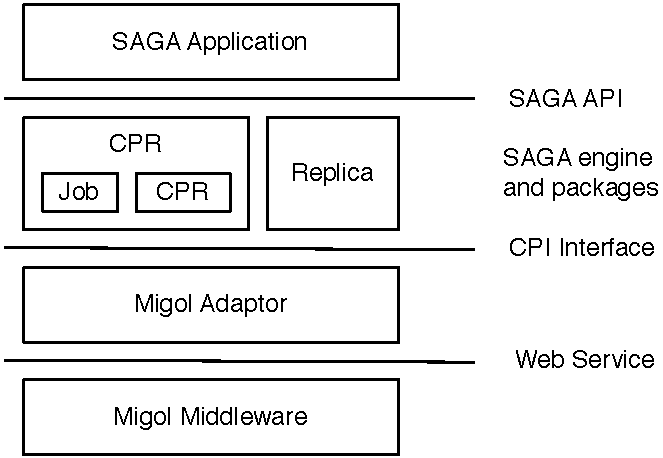
\includegraphics[width=0.6\textwidth]{saga-migol-layered}
%   \caption{SAGA Adaptor for Migol infrastructure}
%   \label{fig:saga-migol-layered}
% \end{figure}  


% \section{Experiences with a Large-Scale Task-Farming Application in the LONI Grid}
% \label{sec:exp}       
% 
%         
% %do we use checkpoints or do we automatically restart the task
% Figure~\ref{fig:saga-taskfarming} gives an overview about the task farming scenario. All tasks are
% distributed using a script and Migol's Job Broker Service.
% %  Each worker will compute a certain 
% % variation of the graph network. Depending on the graph size, the runtime of a single task  can 
% % be as high as \textbf{TODO}  days. 
% To enable the monitoring of a tasks, each task must initialize a \texttt{saga::session} object 
% before starting the computation.  Then, the Migol adaptor starts and registers the monitoring endpoint. 
% %TODO what is the task size/runtime of a single task
% The MRS can now monitor the application.  For error detection we use a timeout of 5 minutes.
% \begin{figure}[t]
%     \centering
%         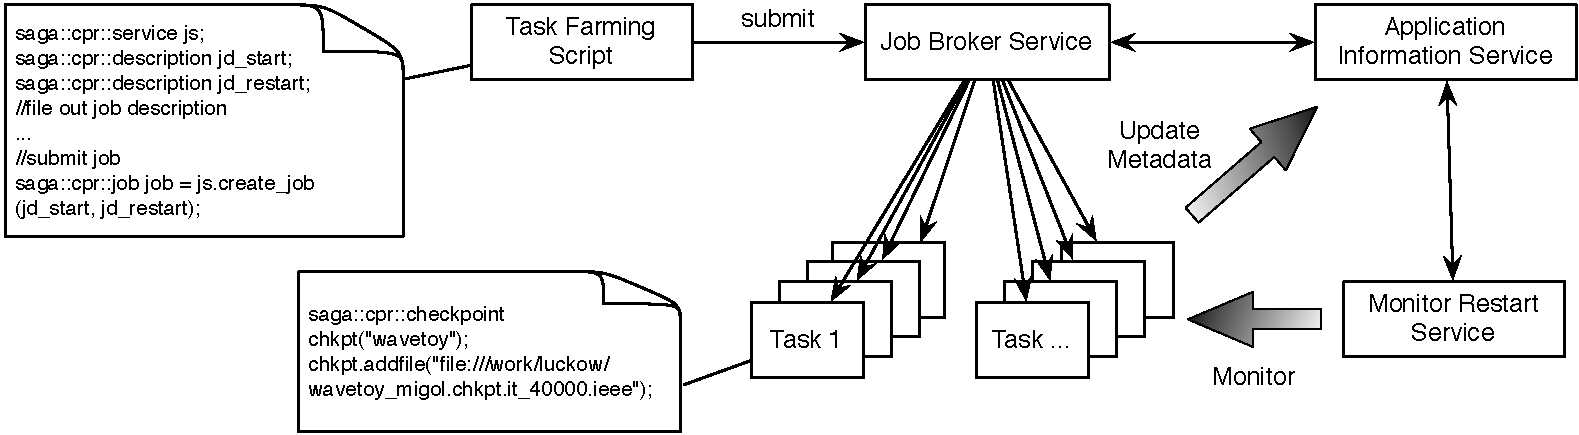
\includegraphics[width=\textwidth]{saga-taskfarming}
%     \caption{Fault Tolerant Task Farming Scenario}
%     \label{fig:saga-taskfarming}
% \end{figure}
% 
% 
% 
% 
%   
% 
% During the runtime, we simulate the failure of a number of worker
% processes.  The Migol MRS successfully detects the respective faults
% and recovers the worker nodes correctly. Even with a high failure
% rate, we were able to obtain the results of our computation.
